\documentclass[margin=0px]{article}

\usepackage{listings}
\usepackage[utf8]{inputenc}
\usepackage{graphicx}
\usepackage{float}
\usepackage[a4paper, margin=0.7in]{geometry}
\usepackage{amsthm}
\usepackage{amssymb}
\usepackage{fancyhdr}
\usepackage{setspace}

\onehalfspacing

\renewcommand{\figurename}{ábra}
\makeatletter
\renewcommand\paragraph{%
    \@startsection{paragraph}{4}{0mm}%
    {-\baselineskip}%
    {.5\baselineskip}%
    {\normalfont\normalsize\bfseries}}
\makeatother
\renewcommand{\figurename}{ábra}
\newenvironment{tetel}[1]{\paragraph{#1 \\}}{}

\pagestyle{fancy}
\lhead{\it{PTI BSc Záróvizsga tételek}}
\rhead{10. Programnyelvi alapok}

\title{\textbf{{\Large ELTE IK - Programtervező Informatikus BSc} \vspace{0.2cm} \\ {\huge Záróvizsga tételek}} \vspace{0.3cm} \\ 10. Programnyelvi alapok}
\author{}
\date{}

\begin{document}
\maketitle

\begin{tetel}{Programnyelvi alapok}
    Fordítás és szerkesztés, programozási nyelv szabályrendszere. Lexikális elemek, szintaxis, szemantikus szabályok. Kifejezések kiértékelésének szabályai. Utasítások, vezérlési szerkezetek. Alaptípusok ábrázolása. Összetett típusok. Programszerkezet, hatókör, láthatóság. Változók ábrázolása a memóriában, élettartam. Paraméterátadás. Kivételek.
\end{tetel}

\section{Fordítás és Interpretálás}

\subsection{Fordítás}

A fordítás során általában egy magas szintű programozási nyelvből gépi kód keletkezik, amelyet a processzor már képes értelmezni és futtatni. Előnye, hogy gyors, mivel a lexikális, szintaktikus és szemantikus elemzés fordítási időben, egyszer fut le, valamint ekkor optimalizáljuk a kódot. Fordítási időben sok hibát ki lehet szűrni, ezáltal megkönnyítve a debugolást. A gépi kód nehezen visszafejthető. Általában nagyobb programokhoz használjuk, ahol fontos a hatékonyság. A lefordított kódon később már nem (vagy csak nagyon nehezen) tudunk változtatni.

Hátránya, hogy a keletkezett kód nem platformfüggetlen, minden architektúrára külön-külön le kell fordítani.

\textbf{Példák}: C, C++, Ada, Haskell

\begin{figure}[H]
    \centering
    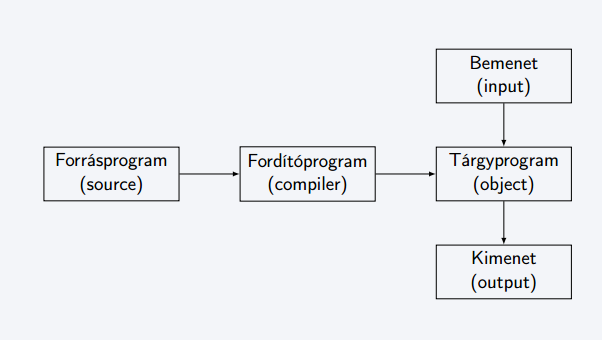
\includegraphics[width=0.5\textwidth]{img/forditas_folyamatabra.png}
    \caption{a fordítás folyamata}
    \label{fig:forditas_folyamatabra}
\end{figure}


\subsection{Interpretálás}

Az interpretálás során a programkódot az értelmező futás közben hajtja végre. Platformfüggetlen, csak az interpretert kell minden rendszerre egyszer megírni. Nehéz benne a hibakeresés, mivel sok olyan hiba maradhat a kódban, amit egy fordító kiszűrt volna (pl. típus egyezőség).

\textbf{Példák}: PHP, JavaScript, ShellScript


\begin{figure}[H]
    \centering
    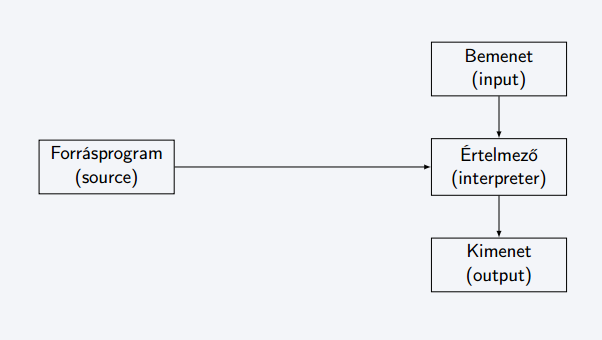
\includegraphics[width=0.5\textwidth]{img/interpretalas_folyamatabra.png}
    \caption{az interpretálás folyamata}
    \label{fig:interpretalas_folyamatabra}
\end{figure}


\subsection{Fordítás és Interpretálás együtt}

Egyes nyelvek (pl. Java) előfordítást használnak, melynek eredménye a \textit{bájtkód}, amely gépi kód egy virtuális gép számára. Ezzel elérhető a fordítási idejű hibaellenőrzés és optimalizálás, de megmarad a platformfüggetlenség.

\begin{figure}[H]
    \centering
    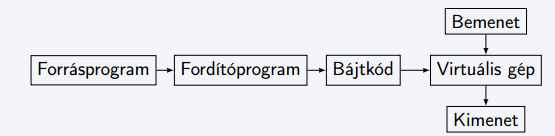
\includegraphics[width=0.5\textwidth]{img/bajtkod_folyamatabra.png}
    \caption{az interpretálás folyamata}
    \label{fig:bajtkod_folyamatabra}
\end{figure}

\section{Fordítási egység és a szerkesztés}

A tárgykód létrehozása két fázisban történik. Először a forrásfájlokat \textit{lefordítjuk}, ebből keletkezik az un. \textit{objektumkód} (pl.: .obj, .class). Ebben a gépi utasítások már megvannak, de hiányzik belőle a hivatkozások (pl változók, függvények), melyek más fájlokban vannak megvalósítva. \textit{Fordítási egységnek} nevezzük azt, amiből egy objektumkód keletkezik.

A \textit{linker} (szerkesztő) feladata, hogy a hiányzó referenciákat kitöltse, hogy egyetlen fájlt generálva futtatható kódot kapjunk.

A linkelés lehet statikus, amikor a fordító tölti fel a hiányzó referenciákat; vagy dinamikus, mikor fordítási időben, jellemzően egy másik fájlból (pl.: .dll) tölti be a hiányzó kódot. Az utóbbi akkor praktikus, ha egy modult több, különálló program használ.


\section{A fordítóprogram komponensei}
\begin{figure}[H]
    \centering
    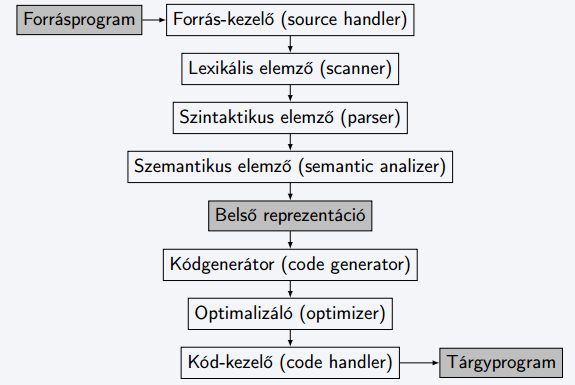
\includegraphics[width=0.5\textwidth]{img/forditas_teljes_folyamata.png}
    \caption{a fordítás lépései}
    \label{fig:forditas_teljes_folyamatabra}
\end{figure}


\subsection{Lexikális elemző}

Bemenete maga a forráskód. A lexikális elemző feladata, hogy tokenekre bontsa a forráskódot. Adott egy reguláris (hármas típusú) nyelvtan, mely a nyelvre jellemző. Ez adja meg,  hogy milyen típusú tokenek szerepelhetnek a forrásban. A tokenekhez tulajdonságokat rendelhet (pl. változó neve, literál értéke). Kimenete ez a tokensorozat. Amennyiben az elemző olyan karaktersorozatot talál, amelynek nem feleltethető meg token, akkor az lexikális hibát vált ki.

\textit{megjegyzés: Lexikális hibánál nem feltétlen szakad meg a fordítás folyamata, megpróbálhatjuk átugrani az adott részt és folytatni az elemzést, így ha több hiba is van, akkor azokat egyszerre jelezhetjük.}

A reguláris kifejezéseket \textit{véges determinisztikus automatákkal} ismerjük fel. Amennyiben egy lexikális elemre az egyik automata elfogadó állapotba kerül, úgy felismertünk egy tokent. Egy karaktersorozatot egyszerre több automata is felismerhet. Amennyiben ezek azonosan hosszúak, akkor a nyelv konfliktusos. Ennek nem szabad előfordulnia. Az viszont lehetséges, hogy egy szót, és az ő prefixét is felismerte egy automata. Ekkor mindig a hosszabbat választjuk.

\subsection{Szintaktikus elemző}

Bemenete a lexikális elemző kimenete. Feladata, hogy \textit{szintaxisfát} építsen a tokenekből, a nyelvez tartozó egy környezetfüggetlen (kettes típusú) grammatika alapján, vagy ha ez lehetetlen, akkor jelezze ezt \textit{szintaktikus hiba}ként.

\subsubsection{LR0 elemzés}

A lexikális elemző által előállított szimbólumsorozatot balról
jobbra olvassuk, a szimbólumokat az elemző vermébe tesszük.

\textit{Léptetés}: egy új szimbólumot teszünk a bemenetről a verem
tetejére.

\textit{Redukálás}: a verem tetején lévő szabály-jobboldalt
helyettesítjük a szabály bal oldalán álló nemterminálissal

A háttérben egy véges determinisztikus automata működik:
az automata átmeneteit a verem tetejére kerülő szimbólumok
határozzák meg
ha az automata végállapotba jut, redukálni kell
egyéb állapotban pedig léptetni.

Az automata bizonyos nyelvek esetén konfliktusos lehet: nem tudjuk eldönteni, hogy léptessünk vagy redukáljunk.

\subsubsection{LR1 elemzés}

Az előző problémára kínál megoldást, kibővítve a lehetséges nyelvek halmazát.

Az ötlet, hogy \textit{olvassunk előre} egy szimbólumot.

Ha az aktuális állapot \textit{i}, és az előreolvasás eredménye az a
szimbólum:

ha $ [A	\rightarrow \alpha.a\beta, b] \in I_i $ és $read(I_i, a) = I_j$
akkor léptetni kell, és átlépni a \textit{j} állapotba.


ha $ [A	\rightarrow \alpha., a] \in I_i (A \neq S'), $
akkor redukálni kell az $ A \rightarrow \alpha $ szabály szerint.




ha $ [S' \rightarrow S., \#] \in I_i $ és $ a = \# $, akkor el kell fogadni a szöveget,	minden más esetben hibát kell jelezni.

Ha az \textit{i} állapotban \textit{A} kerül a verem tetejére:
ha$  read(I_i,A) =	I_j $ ,
akkor át kell lépni a \textit{j} állapotba,	egyébként hibát kell jelezni.



\subsubsection{Jelmagyarázat/Kanonikus halmazok}

\paragraph{Closure/lezárás}

Ha $ I $ a grammatika egy $ LR(1) $ elemhalmaza, akkor $ closure(I) $ a
legszűkebb olyan halmaz, amely az alábbi tulajdonságokkal
rendelkezik:

$ I \subseteq closure(I) $ ha $ [A \rightarrow \alpha.B\gamma,a] \in closure(I) $,

és $ B \rightarrow \beta $ a grammatika egy szabálya,
akkor $ \forall b \in FIRST1(\gamma{}a) $ esetén $ [B \rightarrow .\beta,b] \in closure(I) $


\paragraph{Read/olvasás}
Ha $ I $ a grammatika egy $ LR(1) $ elemhalmaza, $ X $ pedig terminális	vagy nemterminális szimbóluma, akkor $ read(I, X) $ a legszűkebb olyan halmaz, amely az alábbi tulajdonsággal rendelkezik:

Ha $ [A \rightarrow \alpha. X\beta,a] \in I $, akkor $ closure([ A \rightarrow \alpha X.\beta,a]) \subseteq read(I, X) $.


\paragraph{LR(1) kanonikus halmazok ($ I_n $)}
\begin{itemize}
    \item
          $ closure([S' \rightarrow .S, \#]) $ a grammatika egy kanonikus halmaza.
    \item
          Ha $ I $ a grammatika egy kanonikus elemhalmaza, $ X $ egy terminális vagy nemterminális szimbóluma, és $ read(I, X) $ nem üres, akkor $ read(I, X) $ is a grammatika egy kanonikus halmaza.
    \item
          Az első két szabállyal az összes kanonikus halmaz előáll.
\end{itemize}




\subsection{Szemantikus elemző}


A szemantikus elemzés jellemzően a környezetfüggő ellenőrzéseket
valósítja meg.

%Dévai diáiról
\begin{itemize}
    \item
          deklarációk kezelése: változók, függvények, eljárások, operátorok, 	típusok
    \item
          láthatósági szabályok
    \item
          aritmetikai ellenőrzések
    \item
          a program szintaxisának környezetfüggő részei
    \item
          típusellenőrzés
    \item
          stb.
\end{itemize}


A szemantikus elemzéshez ki kell egészítenünk a grammatikát. Rendeljünk a szimbólumokhoz attribútumokat és a szabályokhoz akciókat! Egy adott szabályhoz tartozó feltételek csak a szabályban	előforduló attribútumoktól függhetnek.	(Ha egy feltétel nem teljesül, akkor szemantikus hibát kell	jelezni!). A szemantikus rutinok csak annak a szabálynak az	attribútumait használhatják és számíthatják ki, amelyikhez az őket reprezentáló akciószimbólum tartozik. Minden szintaxisfában minden attribútumértéket pontosan egy
szemantikus rutin határozhat meg. Az így létrejövő nyelvtant \textit{attribútum fordítási grammatikának} (ATG) hívjuk.

A \textit{jól definiált attribútum fordítási grammatika}, olyan attribútum fordítási grammatika, amelyre igaz, hogy a	grammatika által definiált nyelv mondataihoz tartozó minden szintaxisfában minden attribútum értéke egyértelműen kiszámítható.

Egy attribútumot kétféleképpen lehet meghatározni:

\paragraph{Szintézissel} a szintaxisfában alulról felfelé terjed az információ, egy szülő attribútumát a gyerekekből számoljuk. Kitüntetettnek hívjuk azokat az attribútumokat, melyeket a lexikális elemző szolgáltat.

\paragraph{Öröklődéssel} a szintaxisfában felülről lefelé terjed az információ. A gyerekek attribútumait a szülőé határozza meg.

Az \textit{L-ATG} olyan attribútum fordítási grammatika, amelyben minden
$ A	\rightarrow	X_1X_2 . . .	X_n  $szabályban az attribútumértékek az alábbi sorrendben meghatározhatók:

\begin{itemize}
    \item
          A örökölt attribútumai
    \item
          $ X_1 $ örökölt attribútumai
    \item
          $ X_1 $ szintetizált attribútumai
    \item
          $ X_2 $ örökölt attribútumai
    \item
          $ X_2 $ szintetizált attribútumai
    \item
          \dots
    \item
          $ X_n $ örökölt attribútumai
    \item
          $ X_n $ szintetizált attribútumai
    \item
          A szintetizált attribútumai
\end{itemize}

Amennyiben a nyelvtanunk ennek eleget tesz, úgy hatékonyan meghatározható minden attribútum.

A szemantikus elemzéshez jellemzően szimbólumtáblát használunk, verem szerkezettel és keresőfával vagy hash-táblával. Minden blokk egy új szint a veremben, egy szimbólum keresése a verem tetejéről indul.

\section{Kifejezések kiértékelésének szabályai}

\noindent Fogalmak:
\begin{itemize}
    \item	Operandusok: Változók, konstansok, függvény- és eljáráshívások.

    \item	Operátorok: Műveleti jelek, amelyek összekapcsolják egy kifejezésben az operandusokat és valamilyen
          műveletet jelölnek.

    \item	Kifejezés: operátorok és operandusok sorozata

    \item	Precedencia: A műveletek kiértékelési sorrendjét határozza meg.

    \item	Asszociativitás iránya: Az azonos precedenciájú operátorokat tartalmazó kifejezésekben a kiértékelés iránya.
          Megkülönböztetünk bal-asszociatív és jobb-asszociatív operátorokat.
\end{itemize}

\noindent Az operátorokat háromféleképpen írhatjuk az operandusokhoz képest:

\begin{itemize}
    \item	Infix : Egy operátort a két operandusa közé kell írni (tehát csak kétoperandusú műveletek operátorait
          lehet így írni).
          Amikor egy kifejezésben több operátor is szerepel, akkor a különböző operátorok végrehajtási
          sorrendjét az operátorok precedenciája dönti el. Amelyik operátor precedenciája magasabb (pl. a
          szorzásé magasabb, mint az összeadásé), az általa jelölt műveletet értékeljük ki először. Ugyanazon
          operátorok végrehajtási sorrendjét pedig az asszociativitás iránya dönti el (pl. a bal-asszociatív azt
          jelenti, hogy balról jobbra haladva kell végrehajtani). Ezeket a (programozási nyelvekbe beépített)
          szabályokat zárójelek segítségével lehet felülírni.\\
          Példa: A * (B + C) / D

    \item	Postfix (Lengyelforma) : Az operátorokat az operandusaik mögé írjuk. A kiértékelés sorrendje mindig balról jobbra
          történik – tehát egy n operandusú operátor a tőle balra levő első n operandusra érvényes.\\
          Példa: A B C + * D /\\
          Ugyanez zárójelezve (felesleges): ((A (B C +) *) D /)

    \item	Prefix : Az operátorokat az operandusuk elé írjuk. A kiértékelés sorrendje balról
          jobbra történik.\\
          Példa: / * A + B C D\\
          Ugyanez zárójelezve (felesleges): (/ (* A (+ B C) ) D)\\
          Habár a prefix operátorok esetén is balról jobbra történik a kiértékelés, viszont ha egy operátortól
          jobbra egy másik operátor következik, akkor értelemszerűen az ehhez az operátorhoz tartozó
          műveletet kell először végrehajtani, hogy a bal oldalit is végre tudjuk hajtani. A fenti példában is a
          szorzást az osztás előtt, az összeadást pedig a szorzás előtt kell elvégezni.
\end{itemize}

\paragraph{Logikai operátorokat tartalmazó kifejezések kiértékelése}

\noindent Az ilyen kifejezéseknek kétféle kiértékelése létezik:
\begin{itemize}
    \item	Lusta kiértékelés : Ha az első argumentumból meghatározható a kifejezés értéke, akkor a másodikat
          már nem értékeli ki.
    \item	Mohó kiértékelés : Mindenféleképpen megállapítja mindkét argumentum logikai értékét.
\end{itemize}

\noindent A két kiértékelési módszer bizonyos esetekben különböző eredményt adhat:
\begin{itemize}
    \item	A 2. argumentum nem mindig értelmes\\
          Példa (C++):
          \begin{verbatim}
            if ((i>=0) && (T[i]>=10))
            {
                //...
            }
            \end{verbatim}
          Tegyük fel, hogy a T egy \texttt{int} tömb, 0-tól indexelődik.
          Itt ha az $i>=0$ hamis, akkor T-t alul indexelnénk. Ez mohó kiértékelés esetén futási idejű hibát okozna.
          Lusta kiértékelés esetén (a C++ alapértelmezetten ezt használja) viszont tudhatjuk, hogy a feltétel már nem lehet igaz, emiatt $T[i]>=10$-et már nem	kell kiértékelni.
    \item	A 2. argumentumnak van valamilyen mellékhatása.\\
          Példa (C++):
          \begin{verbatim}
            if ((i>0) || (++j>0)) 
            {
                T[j] = 100;
            }
            \end{verbatim}
          Ebben az esetben ha $i>0$ igaz, akkor a feltétel biztosan igaz, viszont a $++j>0$ kifejezés mellékhatásos, növeli j értékét.
          Mivel a C++ lusta kiértékelést használ a $||$ operátor esetén ($|$ operátor esetén mohó a kiértékelés), ezért ebben az esetben nem növeli j értékét. (csak akkor, ha $i>0$ hamis).
\end{itemize}

\section{Utasítások, vezérlési szerkezetek}

\subsection{Egyszerű utasítások}

\begin{itemize}
    \item	Értékadás : Az értékadás bal oldalán egy változó, a jobb oldalán bármilyen kifejezés állhat. Az
          értékadással a változóhoz rendeljük a jobb oldali kifejezést. Figyelni kell arra, hogy a bal oldali
          változó típusának megfelelő kifejezés álljon a jobb oldalon (vagy létezik implicit konverzió, pl. C++-ban
          az egész és logikai típus között). A legtöbb nyelvben az értékadás operátora az \texttt{=} (például C++, Java, C\#),
          vagy a \texttt{:=} (például Pascal, Ada).

    \item	Üres utasítás : Nem mindenhol lehet ilyet írni. A lényege, hogy nem csinál semmit.
          Azokban a nyelvekben lehet létjogosultsága,	ahol üres blokkot nem írhatunk,
          muszáj legalább 1 utasításnak szerepelnie benne. (pl. Ada) Erre szolgál az üres utasítás.
          (Ada-ban ez a \texttt{null} utasítás)

    \item	Alprogramhívás : Alprogramokat nevük és paramétereik megadásával hívhatunk.
          Példák:
          \begin{itemize}
              \item	\texttt{System.out.println("Hello”);}
              \item	\texttt{int x = sum(3,4);}
          \end{itemize}
    \item	Visszatérés utasítás : Az utasítás hatására az alprogram végrehajtása befejeződik. Ha az alprogram egy
          függvény, akkor meg kell adni a visszatérési értéket is.

          \noindent Példák (C++):
          \begin{itemize}
              \item	Ebben a példában a \texttt{doSomething} egy eljárás, nincs visszatérési értéke. A paraméterül kapott
                    x változót értékül adjuk a j-nek. Ha ez az érték nem 0, akkor visszatérünk, azaz megszakítjuk az alprogram
                    végrehajtását (konkrét értéket viszont nem adunk vissza). Ha ez az érték 0, akkor a végrehajtás folytatódik tovább,
                    meghívjuk a \texttt{doSomethingElse} függvényt a j paraméterrel.
                    \begin{verbatim}
            void doSomething(int x)
            {
                int j;
                if(j=x) 
                    return; // j!=0, do nothing
            
                doSomethingElse(j);
            }
            \end{verbatim}

              \item Ebben a példában az \texttt{isOdd} egy függvény, \texttt{int} visszatérési értékkel. Megmondja a paraméterül kapott
                    x egész számról, hogy páratlan-e. Ehhez bitenkénti ÉS művelettel "összeéseli" az x-et az 1-gyel (0...01). Ha az eredmény
                    nem 0, akkor páratlan, visszatérünk igaz értékkel. Különben folytatjuk a működést, majd visszatérünk hamis értékkel.
                    \begin{verbatim}
            int isOdd(int x)
            {
                if(x & 1) //bitwise AND with 0...01 is not 0...0
                    return true;
                    
                return false;
            }
            \end{verbatim}
          \end{itemize}

    \item	Utasításblokk: A blokkon belüli utasítások "összetartoznak”.
          Ez több esetben is jól alkalmazható nyelvi elem:
          \begin{itemize}
              \item	Vezérlési szerkezetekben: Az adott vezérlési szerkezetekhez tartozó utasításokat különíthetjük el.

              \item	Az olyan nyelvekben, amelyekben deklaráció csak a program elején található deklarációs
                    blokkokban lehetséges (pl. Ada), van lehetőség arra, hogy a programkód későbbi részében nyissunk
                    egy blokkot, ahol deklarációk is szerepelhetnek.

              \item	Osztályok inicializáló blokkja pl. Java-ban (konstruktor előtt hajtódik végre):
                    \begin{verbatim}
            public class MyClass{
                private ResourceSet resourceSet;
            
                {
                    resourceSet = new ResourceSetImpl();
                    UMLResourcesUtil.init(resourceSet);
                }
                
                /* ...   */
            }
            \end{verbatim}
              \item	Osztályok statikus inicializáló blokkja pl. Java-ban:
                    \begin{verbatim}
            public class MyClass{
                private static ResourceSet resourceSet;
                
                static{
                    resourceSet = new ResourceSetImpl();
                    UMLResourcesUtil.init(resourceSet);
                }
                
                /*  ...   */
            }
            \end{verbatim}

          \end{itemize}

\end{itemize}

\subsection{Vezérlési szerkezetek}

\begin{itemize}
    \item	Elágazás : Az elágazás egy olyan vezérlési szerkezet, amellyel meghatározhatjuk, hogy bizonyos
          (blokkban megadott) utasítások csak a megadott feltétellel jöhessenek létre.
          Általában több feltételt is megadhatunk egymás után (if L1 then … else if L2 then … else if L3 then …).
          Megadhatjuk azt is, hogy mi történjen, ha egyik feltétel sem teljesül (if L then … else …).

          Elágazásokat lehet egymásba ágyazni (if … then if ...).

          "Csellengő else” ("Dangling else”) probléma: Azokban a nyelvekben lép fel, ahol egy feltétel egy
          utasításblokkját nem zárja le külön kódszó (pl. endif). Ekkor abban az esetben, ha elágazásokat
          egymásba ágyazunk, a következő probléma léphet fel:\\
          Példa: \texttt{if (A>B) then if (C>D) then E:=100; else F:=100;}

          A fenti esetben nem lehet megállapítani, hogy a programozó az else kulcsszót melyik elágazásra
          értette.

    \item	Ciklus : Egy utasításblokk (ciklusmag) valahányszori végrehajtását jelenti.
          \begin{itemize}
              \item	Feltétel nélküli ciklus : Végtelen ciklust kódol, kilépni belőle a strukturálatlan utasításokkal lehet
                    (ld. lentebb), vagy return-nel, esetleg hiba fellépése esetén.

                    Példa (ADA):
                    \begin{verbatim}
                    loop
                        null;
                    end loop;
                \end{verbatim}

              \item	Elöltesztelő ciklus : A ciklus a ciklusmag minden végrehajtása előtt megvizsgálja, hogy az adott
                    feltétel teljesül-e. Ha teljesül, akkor végrehajtja a magot, majd újra ellenőriz. Különben a ciklus
                    után folytatódik a futás.

                    Példák:
                    \begin{itemize}
                        \item	C++:
                              \begin{verbatim}
                    int x=0,y=0;
                    while(x<5 && y<5)
                    {
                        x+=y+1;
                        y=x-1;
                    }
                    cout<<x+y<<endl;
                \end{verbatim}

                        \item	ADA:
                              \begin{verbatim}
                    declare
                        X,Y: Integer;
                    begin
                        X:=0;
                        Y:=0;
                        while X<5 and Y<5 loop
                            X:=X+Y+1;
                            Y:=X-1;
                        end loop;
                    end;
                \end{verbatim}
                    \end{itemize}

              \item	Számlálásos ciklus : Ebben a vezérlési szerkezetben megadhatjuk, hogy a ciklusmag hányszor
                    hajtódjon végre.
                    Példa (ADA):
                    \begin{verbatim}
                for i in 1..10 loop 
                    null;
                end loop;
            \end{verbatim}
                    A számlálás úgy történik, hogy egy változóban (ciklusváltozó) tároljuk, hogy "hol tartunk” - ezt hasonlítjuk
                    össze minden ciklus elején a kifejezéssel, amit meg kell haladnia a változónak (i). Tehát
                    felfogható egy elöltesztelő ciklusként is, ahol a ciklusfeltétel az \texttt{i<=10} és a ciklusmag végén
                    növelni kell i-t.

              \item	Hátultesztelő ciklus : Az a különbség az elöltesztelőhöz képest, hogy a feltételt a ciklusmag
                    végrehajtása után ellenőrizzük – tehát itt a ciklusmag 1-szer mindenképpen lefut.

                    Példa (C++):

                    \begin{verbatim}
                int i=0;
                do
                {
                    ++i;
                } while(i<5);
            \end{verbatim}

                    Megjegyzés: vannak olyan nyelvek (pl. Pascal), amelyekben a hátultesztelő ciklus feltétele nem bennmaradási, hanem
                    leállási feltétel. Azaz nem azt adjuk meg, hogy minek kell teljesülnie ahhoz, hogy még egyszer végrehajtásra kerüljön
                    a ciklusmag, hanem azt, hogy minek kell teljesülnie ahhoz, hogy a ciklusmag ne hajtódjon végre többször.

                    Az előbbi C++-os példa Pascal-os megfelelője:
                    \begin{verbatim}
                i:=0;
                repeat
                    i:=i+1;
                until i=5;
            \end{verbatim}

                    Megjegyzés: ADA-ban nincs igazi hátultesztelős ciklus. Ebben a nyelvben hátultesztelő ciklust úgy írhatunk, hogy ha
                    írunk egy feltétel nélküli ciklust, amelynek utolsó utasítása egy feltételhez kötött kilépés.

                    Példa:
                    \begin{verbatim}
                i:=0;
                loop
                    i:=i+1;
                    exit when i=5;
                end loop;
            \end{verbatim}


              \item	foreach : Akkor használatos, ha egy adatszerkezet minden elemére végre akarjuk hajtani a magot.
                    Tulajdonképpen ez is egy elöltesztelő ciklus (a ciklusfeltétel az, hogy a végére értünk-e az
                    adatszerkezetnek).
                    Példa:
                    \begin{verbatim}
                foreach (int v in Vect)
                {
                    ++v;
                }
            \end{verbatim}

                    Megjegyzések:
                    \begin{enumerate}
                        \item	Nincs minden programozási nyelvben ilyen ciklus. Leginkább az újabb nyelvekben terjedt el.
                        \item	Nem minden programozási nyelvben a foreach a kulcsszó ehhez a ciklushoz.
                              Például Java-ban, C++11-ben (régebbi változatokban nincs ilyen) a for ciklust használhatjuk foreach-ként:
                              \begin{verbatim}
                int x=0;
                for (int v : vect){
                    x+=v;
                }
                \end{verbatim}
                    \end{enumerate}

          \end{itemize}
\end{itemize}

\subsection{Strukturálatlan utasítások}

\begin{itemize}
    \item	Ciklus megszakítása : A ciklusból való "kiugrásra” (tehát annak azonnali befejezésére) használható.
          Gyakran végtelen ciklus megszakítására használjuk, vagy hátultesztelő ciklus kódolására (ahol nincs
          erre beépített vezérlési szerkezet, például Ada).

          Ilyen utasítás pl. C/C++/C\#-ban, vagy Java-ban a \texttt{break}, illetve Ada-ban az \texttt{exit}.

    \item	\texttt{goto} utasítás : A programkódban címkéket definiálhatunk, majd a \texttt{goto} utasítással egy
          ilyen címkéhez irányíthatjuk a vezérlést. Vezérlési szerkezeteket is lehet vele kódolni. Túlzott
          használata olvashatatlan kódhoz vezethet.
\end{itemize}

\subsection{Rekurzió}

Rekurzív alprogram: Olyan alprogram, amelynek kódjában szerepel önmagának a meghívása.
Mindenképpen kell, hogy legyen a rekurziónak megállási feltétele – tehát egy olyan feltétel (egy elágazással
együtt), amelynek teljesülése esetén nem történik rekurzív hívás, így az összes, folyamatban levő rekurzív hívás
végre tud hajtódni (ellenkező esetben végtelen rekurzió lép fel, ilyenkor általában előbb-utóbb betelik a stack és leáll a program).\\

\noindent Példák (faktoriális):

\begin{itemize}
    \item	C++:
          \begin{verbatim}
            int fact (int n)
            {
                if(n>0)
                    return n * fact (n-1);
                else
                    return 1;
            }
        \end{verbatim}

    \item	Haskell:
          \begin{verbatim}
            fact :: (Integral a) => a -> a  
            fact n
                | n>0 = n * fact (n - 1)  
                | otherwise = 0
        \end{verbatim}

\end{itemize}

\section{Kódgenerálás alapvető vezérlési szerkezetekhez}


A kódgenerálás feladata, hogy a szintaktikusan és szemantikusan elemzett programot tárgykóddá alakítsa. Általában szorosan összekapcsolódik a
szemantikus elemzéssel.

\subsection{Értékadás}

assignment $ \rightarrow $ variable assignmentOperator expression

\begin{verbatim}
		a kifejezést az eax regiszterbe kiértékelö kód
		2 mov [Változó],eax
	\end{verbatim}

\subsection{Egy ágú elágazás}
statement $ \rightarrow $ if condition then program end

\begin{verbatim}
		1 a feltételt az al regiszterbe kiértékelö kód
		2 cmp al,1
		3 je Then
		4 jmp Vége
		5 Then: a then-ág programjának kódja
		6 Vége:
	\end{verbatim}

\textit{megjegyzés: a dupla ugrásra azért van szükség, mert a feltételes ugrás hatóköre limitált.}

\subsection{Több ágú elágazás}


statement $ \rightarrow $
\\if $ condition_1 $ then $ program_1 $
\\elseif $ condition_2 $ then $ program_2 $
\\\dots
\\elseif $ condition_n $ then $ program_n $
\\else $ program_{n+1} $ end

\begin{verbatim}
		1 az 1. feltétel kiértékelése az al regiszterbe
		2 cmp al,1
		3 jne near Feltétel_2
		4 az 1. ág programjának kódja
		5 jmp Vége
		6
		...
		7 Feltétel_n: az n-edik feltétel kiértékelése az al regiszterbe
		8 cmp al,1
		9 jne near Else
		10 az n-edik ág programjának kódja
		11 jmp Vége
		12 Else: az else ág programjának kódja
		13 Vége:
	\end{verbatim}

\subsection{Switch-case}
statement $ \rightarrow $ switch variable
\\case $ value_1 $ : $ program_1 $
\\...
\\case $ value_n $ : $ program_n $

\begin{verbatim}
		1 cmp [Változó],Érték_1
		2 je near Program_1
		3 cmp [Változó],Érték_2
		4 je near Program_2
		5
		. ..
		6 cmp [Változó],Érték_n
		7 je near Program_n
		8 jmp Vége
		9 Program_1: az 1. ág programjának kódja
		10
		. ..
		11 Program_n: az n-edik ág programjának kódja
		12 Vége:
	\end{verbatim}

\subsection{Ciklus}
%Ez egy vagy két szó?
\subsubsection{Elől tesztelő}
statement $ \rightarrow $ while condition statements end

\begin{verbatim}
		1 Eleje: a ciklusfeltétel kiértékelése az al regiszterbe
		2 cmp al,1
		3 jne near Vége
		4 a ciklusmag programjának kódja
		5 jmp Eleje
		6 Vége:
	\end{verbatim}


%Ez egy vagy két szó?
\subsubsection{Hátul tesztelő}
statement $ \rightarrow $ loop statements while condition


\begin{verbatim}
		1 Eleje: a ciklusmag programjának kódja
		2 a ciklusfeltétel kiértékelése az al regiszterbe
		3 cmp al,1
		4 je near Eleje
	\end{verbatim}

\subsubsection{For ciklus}

statement $ \rightarrow $ for variable from $ value_1 $ to $ value_2 $ statements end


\begin{verbatim}
		1 a "from" érték kiszámítása a [Változó] memóriahelyre
		2 Eleje: a "to" érték kiszámítása az eax regiszterbe
		3 cmp [Változó],eax
		4 ja near Vége
		5 a ciklusmag kódja
		6 inc [Változó]
		7 jmp Eleje
		8 Vége:
	\end{verbatim}

\subsection{Statikus változók}

Kezdőérték nélküli változódefiníció fordítása:
\begin{verbatim}
		section .bss
		; a korábban definiált változók...
		Lab12: resd 1 ; 1 x 4 bájtnyi terület
	\end{verbatim}


Kezdőértékkel adott változódefiníció fordítása:
\begin{verbatim}
		section .data
		; a korábban definiált változók...
		Lab12: dd 5 ; 4 bájton tárolva az 5-ös érték
	\end{verbatim}

\subsection{Logikai kifejezések}

\subsubsection{kifejezés1 $ < $  kifejezés2 }

\begin{verbatim}
		; a 2. kifejezés kiértékelése az eax regiszterbe
		push eax
		; az 1. kifejezés kiértékelése az eax regiszterbe
		pop ebx
		cmp eax,ebx
		jb Kisebb
		mov al,0 ; hamis
		jmp Vége
		Kisebb:
		mov al,1 ; igaz
		Vége:
	\end{verbatim}

\subsubsection{kifejezés1 $ \lbrace $ és, vagy, nem, kizáróvagy  $ \rbrace $  kifejezés2 }

\begin{verbatim}
		; a 2. kifejezés kiértékelése az al regiszterbe
		push ax ; nem lehet 1 bájtot a verembe tenni!
		; az 1. kifejezés kiértékelése az al regiszterbe
		pop bx ; bx-nek a bl részében van,
		; ami nekünk fontos
		and al,bl
	\end{verbatim}

\subsubsection{ lusta "és" kiértékelés }

\begin{verbatim}
		; az 1. kifejezés kiértékelése az al regiszterbe
		cmp al,0
		je Vége
		push ax
		; a 2. kifejezés kiértékelése az al regiszterbe
		mov bl,al
		pop ax
		and al,bl
		Vége:
	\end{verbatim}


\subsubsection{ Alprogramok megvalósítása }


\begin{verbatim}
		; az 1. kifejezés kiértékelése az al regiszterbe
		cmp al,0
		je Vége
		push ax
		; a 2. kifejezés kiértékelése az al regiszterbe
		mov bl,al
		pop ax
		and al,bl
		Vége:
	\end{verbatim}

\subsubsection{ Alprogramok hívása }

\begin{verbatim}
		Alprogramok sémája
		; utolsó paraméter kiértékelése eax-be
		push eax
		; ...
		; 1. paraméter kiértékelése eax-be
		push eax
		call alprogram
		add esp,’a paraméterek összhossza’
	\end{verbatim}

\section{Kódoptimalizáló}

Az optimalizálás feladata, hogy a keletkezett kód kisebb és gyorsabb legyen, úgy hogy a futás eredménye nem változik. A gyorsaság és a tömörség gyakran ellentmondanak egymásnak, és az egyik csak a másik rovására lehet javítani. Általában három lépésben szokás elvégezni:

\begin{itemize}
    \item
          Optimalizálási lépések végrehajtása az eredeti programon (vagy annak egyszerűsített változatán)
    \item
          Kódgenerálás
    \item
          Gépfüggő optimalizálás végrehajtása a generált kódon
\end{itemize}

\subsection{Lokális optimalizáció}

Egy programban egymást követő utasítások sorozatát \textit{alapblokknak} nevezzük, ha az első utasítás kivételével egyik utasítására sem lehet távolról átadni a vezérlést (assembly programokban: ahová a jmp, call, ret utasítások "ugranak"; magas szintű nyelvekben: eljárások, ciklusok eleje, elágazások ágainak első utasítása, goto utasítások célpontjai). Az utolsó utasítás kivételével nincs benne vezérlés-átadó utasítás (assembly programban: jmp, call, ret magas szintű nyelvekben: elágazás vége, ciklus vége, eljárás vége, goto). Az utasítás-sorozat nem bővíthető a fenti két szabály megsértése nélkül.

Ha az optimalizálás az alapblokkok keretein belül történik, akkor garantált, hogy az átalakításnak nincs mellékhatása. Ez a \textit{lokális optimalizálás}.

\paragraph{Ablakoptimalizálás}
Ez egy módszer a lokális optimalizálás egyes fajtáihoz. Egyszerre csak egy néhány utasításnyi részt vizsgálunk a kódból. A vizsgált részt előre megadott mintákkal hasonlítjuk össze. Ha illeszkedik, akkor a mintához megadott szabály szerint átalakítjuk ezt az "ablakot" végigcsúsztatjuk a programon. Az átalakítások megadása:
\begin{center}
    $ \lbrace$ minta $ \rightarrow $ helyettesítés $\rbrace$ szabályhalmazzal
    (a mintában lehet paramétereket is használni)
\end{center}

Példák:
\begin{itemize}
    \item
          felesleges műveletek törlése: nulla hozzáadása vagy kivonása
    \item
          egyszerűsítések: nullával szorzás helyett a regiszter törlése
    \item
          regiszterbe töltés és ugyanoda visszaírás esetén a visszaírás elhagyható
    \item
          utasításismétlések törlése: ha lehetséges, az ismétlések törlése
\end{itemize}


\subsection{Globális optimalizáció}
A teljes program szerkezetét meg kell vizsgálni. Ennek módszere az adatáram-analízis:
\begin{itemize}
    \item
          Mely változók értékeit számolja ki egy adott alapblokk?
    \item
          Mely változók értékeit melyik alapblokk használja fel?
\end{itemize}


Ez lehetővé teszi az azonos kifejezések többszöri kiszámításának kiküszöbölését akkor is, ha különböző alapblokkokban szerepelnek; valamint a konstansok és változók továbbterjesztését alapblokkok között is elágazások, ciklusok optimalizálását.

\section{A szekvenciális és	párhuzamos/elosztott végrehajtás összehasonlítása}

\subsection{Szekvenciális végrehajtás:}

Ilyenkor a végrehajtás egy processzoron történik. Minden művelet atomi. Egy inputhoz egy output tartozik. Két szekvenciális program ekvivalens, ha ezek a párosok megegyeznek. Nem használja fel az összes rendelkezésre álló erőforrást.


\subsection{Párhuzamos végrehajtás:}

Több processzoron hajtódik végre a program. A párhuzamos folyamatok egymással kommunikálva, szinkronban oldják meg az adott problémát. A konkurens program szétbontható elemi szekvenciális programokra, ezek a folyamatok. A folyamatok használhatnak közös erőforrásokat: pl. változók, adattípus  objektumok, kommunikációs csatornák.

A kommunikációt általában kétféleképpen szokták megvalósítani.
\paragraph{Osztott memóriával.} Ekkor szinkronizálni kell, hogy ki mikor fér hozzá, hogy ne legyen ütközés.

\paragraph{Kommunikációs csatornával.} Garantálni kell, hogy ha egy folyamat üzenetet küld egy másiknak, akkor az meg is kapja azt, és jelezzen is vissza. Ügyelni kell, nehogy deadlock alakuljon ki.


\section{Típusok}

\subsection{Tömb}

A tömb (angolul array) olyan adatszerkezet, amelyet nevesített elemek csoportja alkot, melyekre sorszámukkal (indexükkel) lehet hivatkozni. Vektornak is nevezik, ha egydimenziós, mátrixnak esetenként, ha többdimenziós. A legtöbb programozási nyelvben minden egyes elemnek azonos adattípusa van és a tömb folytonosan helyezkedik el a számítógép memóriájában. A készítés módja alapján lehet:

\begin{itemize}
    \item	statikus :a méret fix, deklarációban szabályozott
    \item	dinamikus tömb: a mérete változik, folyamatosan bővíthető
\end{itemize}

\subsection{Rekord}

A rekord egy összetett értékek leírásához használható konstrukció. Névvel és típussal ellátott összetevői vannak, ezeket mezőknek nevezzük.
Értékhalmaz a mezők értéktípusai által meghatározott alaphalmazok direktszorzata.

\begin{figure}[H]
    \centering
    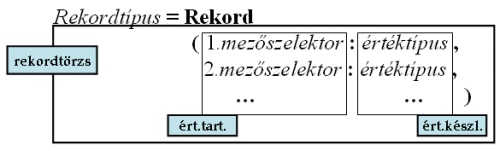
\includegraphics[width=0.7\linewidth]{img/rekord}
    \caption{A rekord-típuskonstrukciók általános szintaxisa.}
    \label{fig:rekord}
\end{figure}

\noindent Műveletek:
\begin{itemize}
    \item	Szelekciós függvény (.mezőszelektor szintaxisú);

    \item	konstrukciós függvény (Rekordtípus(mezőértékek) szintaxisú);

    \item	elképzelhetők transzformációs függvények, amelyek a teljes rekordstruktúrát érintik.
\end{itemize}

\noindent Példa rekordra és használatára C-ben:
\begin{verbatim}
    //definition of Point
    struct Point 
    {
        int xCoord;
        int yCoord;
    };
    
    const struct Point ORIGIN = {0,0};
        
\end{verbatim}

\subsection{Osztály}

Az osztály egy felhasználói típus, amelynek alapján példányok (objektumok)
hozhatók létre. Az osztály alapvetően attribútum és metódus (művelet) definíciókat
tartalmaz. Az osztály írja le az objektum típusát: megadja a tulajdonságait és azok
lehetséges értékeit (azaz a típusértékeket), valamint az objektumon végrehajtható műveleteket (típusműveletek).\\

\noindent Példa C++-ban:
\begin{verbatim}
        //definition of Point
        class Point {
        private:
            int xCoord;
            int yCoord;
        public:
            //constructor
            Point(int xCoord, int yCoord) : xCoord(xCoord),yCoord(yCoord) {}
            
            void Translate(int dx, int dy) {
                xCoord+=dx;
                yCoord+=dy;
            }
            
            void Translate(Point delta) {
                xCoord+=delta.xCoord;
                yCoord+=delta.yCoord;
            }
            
            int getX() { return xCoord; }
            
            int getY() { return yCoord; }
        };
        
        int main(int argc, char* argv[])
        {
            Point point(0,0);
            point.Translate(5,-2);
            cout<<point.getX()<<","<<point.getY()<<endl; //5,-2
            Point delta(-2,1);
            point.Translate(delta);
            cout<<point.getX()<<","<<point.getY()<<endl; //3,-1
            
            return 0;
        }
        \end{verbatim}

Megjegyzés: A nem objektum-orientált nyelvekben nincsenek osztályok, pl. régebbi nyelvekben, mint a C, ADA, Pascal, vagy
funkcionális nyelvekben (Haskell, Clean, stb.).

\subsection{Öröklődés}

Egy osztály legegyszerűbben adattagjainak és metódusainak felsorolásával hozható létre. Azonban az objektum-orientált paradigma lehetőséget ad egy másik, hatékonyabb módszerre is, az öröklődésre. Az öröklődés az újrafelhasználhatóságot szem előtt tartva arra ad lehetőséget, hogy már meglévő (szülő-, ős-) osztályból kiindulva hozzunk létre új (gyermek-, leszármazott-, al-) osztályt. Az öröklés két osztály között fennálló olyan kapcsolat, amely során a leszármazott osztály rendelkezik a szülő osztály majdnem összes tulajdonságával (nem privát adattagjait és metódusait sajátjaként kezeli), s ezeket újabbakkal egészítheti ki. Az így létrehozott osztály is lehet más osztályok őse (kivéve pl. Java-ban a \texttt{final} kulcsszóval ellátott osztályok, ezekből már nem származtathatunk), így ezek az osztályok egy öröklési hierarchiába szerveződnek. Attól függően, hogy egy osztálynak egy- vagy több őse van, beszélünk egyszeres- ill. többszörös öröklődésről. A Java az egyszeres öröklődést támogatja, de pl. C++-ban van többszörös öröklődés.

A Java-ban az osztályhierarchia legfelső eleme az Object osztály, amelyből minden más osztály (közvetve vagy közvetlenül) származik.

Egy alosztály az örökölt metódusokat újraimplementálhatja. Ilyenkor az adott metódus ugyanolyan néven, de más, módosított (alosztályra specifikált) tartalommal kerül megvalósításra. Az ilyen metódusokat polimorfnak nevezzük. Java-ban minden olyan metódust, ami nincs ellátva a \texttt{final} kulcsszóval, újra lehet definiálni. (C++-ban mindent, ami nem privát)\\

\noindent Példák:
\begin{itemize}
    \item	C++:
          \begin{verbatim}
                class RegularPolygon
                {
                protected:
                    const double radius;
                public:
                    RegularPolygon(double radius) : radius(radius) {}
                    virtual double area() = 0;
                };
                
                class EquilateralTriangle : public RegularPolygon
                {
                public:
                    EquilateralTriangle(double radius) : RegularPolygon(radius) {}
                    virtual double area()
                    {
                         return 0.75*sqrt(3.0)*radius*radius;
                    }
                };
            \end{verbatim}

    \item	Java:
          \begin{verbatim}
            public abstract class RegularPolygon{
                protected final double radius;
            
                public RegularPolygon(double radius){
                    this.radius = radius;
                }
                public abstract double area();
            }
            
            public class EquilateralTriangle extends RegularPolygon{
                public EquilateralTriangle(double radius){
                    super(radius);
                }
                public double area(){
                     return 0.75*Math.sqrt(3.0)*radius*radius;
                }
            }
            
            \end{verbatim}
\end{itemize}

\section{Hatókör/láthatóság}

\begin{enumerate}
    \item	Hatókör: Deklarációkor a programozó összekapcsol egy entitást (például egy változót vagy függvényt) egy névvel. A hatókör alatt a forrásszöveg azt a részét értjük, amíg ez az összekapcsolás érvényben van. Ez általában annak a blokknak a végéig tart, amely tartalmazza az adott deklarációt.

    \item	A láthatóság a hatókör részhalmaza, a programszöveg azon része, ahol a deklarált névhez a megadott entitás tartozik. Mivel az egymásba ágyazott blokkokban egy korábban már bevezetett nevet más entitáshoz kapcsolhatunk, ezért ilyenkor a külső blokkban deklarált entitás a nevével már nem elérhető. Ezt nevezzük a láthatóság elfedésének.

          Egyes nyelvekben (például C++) bizonyos esetekben (például osztályszintű adattagok) a külső blokkban deklarált entitáshoz minősített névvel hozzá lehet férni ekkor is.
\end{enumerate}

\section{Automatikus, statikus és dinamikus élettartam, szemétgyűjtés}
Élettartam: A változók élettartama alatt a program végrehajtási idejének azt a szakaszát értjük, amíg a változó számára lefoglalt tárhely a változóé.

\subsection{Automatikus élettartam}

A blokkokban deklarált lokális változók automatikus élettartamúak, ami azt jelenti, hogy a deklarációtól a tartalmazó blokk végéig tart, azaz egybeesik a hatókörrel. A helyfoglalás számukra a végrehajtási verem aktuális aktivációs rekordjában történik meg.

\subsection{Statikus élettartam}

A globális változók, illetve egyes nyelvekben a statikusként deklarált változók (például C/C++ esetén a \texttt{static} kulcsszóval) statikus élettartamúak. Az ilyen változók élettartama a program teljes végrehajtási idejére kiterjed, számukra a helyfoglalás már a fordítási időben megtörténhet.

\subsection{Dinamikus élettartam}

A dinamikus élettartamú változók esetén a programozó foglal helyet számukra a dinamikus tárterületen (heap), és a programozó feladata gondoskodni arról is, hogy ezt a tárterületet később felszabadítsa. Amennyiben utóbbiról megfeledkezik, azt nevezzük memóriaszivárgásnak (memory leak).
Mint látjuk, a dinamikus élettartam esetén a hatókör semmilyen módon nem kapcsolódik össze az élettartammal, az élettartam szűkebb vagy tágabb is lehet a hatókörnél.

\subsection{Szemétgyűjtő}

A szemétgyűjtő másik neve a hulladékgyűjtő, az angol Garbage Collector név után pedig gyakran csak GC-nek rövidítik. Feladata a dinamikus memóriakezeléshez kapcsolódó tárhelyfelszabadítás automatizálása, és a felelősség levétele a programozó válláról, így csökkentve a hibalehetőséget.

A szemétgyűjtő figyeli, hogy mely változók kerültek ki a hatókörükből, és azokat felszabadíthatóvá nyilvánítja. A módszer hátránya a számításigényessége, illetve a nemdeterminisztikussága. A szemétgyűjtő ugyanis nem szabadítja fel egyből a hatókörükből kikerült változókat, és a felszabadítás sorrendje sem ugyanaz, amilyen sorrendben a változók felszabadíthatóvá váltak.

Azt, hogy a hulladékgyűjtő mikor és mely változót szabadítja fel, egy programozási nyelvenként egyedi, összetett algoritmus határozza meg, amelyben rendszerint szerepet játszik a rendelkezésre álló memória telítettsége, illetve a felszabadításhoz szükséges becsült idő. (Például ha egy objektum rendelkezik destruktorral, akkor általában a GC később szabadítja csak fel.)

Összességében a szemétgyűjtő csak annyit garantál, hogy előbb-utóbb (legkésőbb a program futásának végeztével) minden dinamikusan allokált változót felszabadít.

Szemétgyűjtést használó nyelvek pl. Java, C\#, Ada. C/C++-ban nincs szemétgyűjtés, a programozónak kell gondoskodni a dinamikusan allokált memóriaterületek felszabadításáról.

\section{Alprogramok, paraméterátadás, túlterhelés}

\subsection{Alprogramok}

Alprogramoknak a függvényeket, eljárásokat és műveleteket nevezzük. Segítségükkel a program feladatonként tagolható, a főprogramból az önálló feladatok kiszervezhetőek.

\subsection{Paraméterátadás}

Az alprogramoknak szüksége lehet bemenő adatokra és vissza is adhat értékeket. Az alprogramokat általános írjuk meg, saját változónevekkel, ezek a formális paraméterek. Az alprogram meghívásakor az átadott aktuális paraméterek alapján a formális paraméterek értéket kapnak. Az, hogy a formális paraméterek értéke mi lesz, a paraméterátadás módjától függ.

\subsubsection{Szövegszerű paraméterátadás}

A makrókban használatosak mind a mai napig. A makró törzsében a formális paraméter helyére beíródik az aktuális paraméter szövege.

\subsubsection{Név szerinti paraméterátadás}

Az aktuális paraméter kifejezést újra és újra kiértékeljük, ahányszor hivatkozás történik a formálisra. A paramétert a törzs kontextusában értékeljük ki, így a formális paraméter különböző előfordulásai mást és mást jelenthetnek az alprogramon belül.
Alkalmazása archaikus (például: Algol 60, Simula 67).

\subsubsection{Érték szerinti paraméterátadás}

Az egyik legelterjedtebb paraméterátadási mód (például: C, C++, Pascal, Ada, Java), bemeneti szemantikájú. A formális paraméter az alprogram lokális változója, híváskor a vermen készül egy másolat az aktuális paraméterről, ez lesz a formális. Az alprogram végén a formális paraméter megszűnik

\subsubsection{Cím szerinti paraméterátadás}

A másik legelterjedtebb paraméterátadási mód (például: Pascal, C++, C\#), be- és kimeneti szemantikájú. A híváskor az aktuális paraméter címe adódik át, azaz a formális és az aktuális paraméter ugyanazt az objektumot jelentik, egy alias jön létre.\\

Megjegyzés: A Java-ban nincs cím szerinti paraméterátadás, csak érték szerinti. A Java ugyanis a primitív típusoknak az értékét tárolja,
objektumok esetén pedig egy referenciát az adott objektumra (mint C++-ban a referencia típus).  Objektum átadásakor ez a referencia másolódik le, azaz a referencia adódik át érték szerint.\\

\noindent	Például:
\begin{verbatim}
        public static void BadSwap(Object x, Object y)
        {
            Object tmp = x;
            x = y;
            y = tmp;
        }
\end{verbatim}

A fenti függvény nem cseréli ki az x-et és y-t, csak lokálisan (a függvénytörzsön belül), viszont a hívás helyén
x és y is helyben maradnak.

\subsubsection{Eredmény szerinti paraméterátadás}

Kimeneti szemantikájú paraméterátadási mód. A formális paraméter az alprogram lokális változója, az alprogram végén a formális paraméter értéke bemásolódik az aktuálisba. Azonban az alprogram meghívásakor az aktuális értéke nem másolódik be a formálisba. (Használja például az Ada.)

\subsubsection{Érték/eredmény szerinti paraméterátadás}

Az érték és eredmény szerinti paraméterátadás összekombinálása, így egy be- és kimeneti szemantikájú paraméterátadási módot kapunk. (Használja például az Algol-W vagy az Ada.)

\subsubsection{Megosztás szerinti paraméterátadás}

Objektumorientált programozási nyelvek (például: CLU, Eiffel) paraméterátadási módja. Lényege, hogy ha a formális paraméter megváltoztatható és az aktuális paraméter egy megváltoztatható változó, akkor cím szerinti paraméterátadás történik, egyébként pedig érték szerinti. A paraméterátadás módját külön megadni nem lehet.
Megváltoztatható (mutable) objektum alatt azt értjük, hogy tulajdonságai, ezáltal állapota megváltoztatható.

\subsubsection{Igény szerinti paraméterátadás}

Ezt a paraméterátadási módot a lusta kiértékelésű funkcionális nyelvek (például: Clean, Haskell, Miranda) alkalmazzák. Az aktuális paramétert nem híváskor értékeli ki, hanem akkor, amikor először szüksége van rá a számításokhoz.

\subsection{Túlterhelés}

A túlterhelés (overloading) segítségével azonos nevű alprogramokat hozhatunk létre eltérő szignatúrával. A szignatúra a legtöbb programozási nyelvben az alprogram nevét és a formális paraméterek számát és típusát jelenti, de egyes nyelvekben (például Ada) a visszatérési érték típusa is beletartozik. A túlterhelés elsődleges felhasználási területe, hogy ugyanazt a tevékenységet különböző paraméterezéssel is elvégezhessük.

A fordító az alprogramhívásból el tudja dönteni, hogy a túlterhelt változatok közül melyiket kell meghívni. Ha egyik sem illeszkedik vagy több is illeszkedik, akkor fordítási hiba lép fel.

\section{Kivételkezelés}
A kivételkezelés egy programozási mechanizmus, melynek célja a program futását szándékosan vagy nem szándékolt módon megszakító esemény (hiba) vagy utasítás kezelése. Az eseményt magát kivételnek hívjuk. A hagyományos, szekvenciális és strukturált programozási kereteken túlmutató hibakezelésre, valamint magasabb szintű hibadetekcióra, esetleg korrigálásra használható.

Ahhoz, hogy ne maradjanak a hibák kezeletlenül, érdemes nyelvi szinten megkövetelni a hibakezelést. A lényeg, hogy amikor egy hiba megjelenik a programban, azaz egy kivételes esemény történik, a program normális végrehajtása megáll, és átadódik a vezérlés a kivételkezelő mechanizmusnak. Mivel az alapfilozófia úgyis az, hogy a hibás kód nem tud jól működni, amíg a hiba nincs kezelve, nem érdemes folytatni a program végrehajtását. Azzal, hogy a kivételt lekezelő kód elkülönül a normálisan futó kódtól, az az előnyünk is megadatik, hogy maga a kód megtisztul és áttekinthetőbb lesz, nem kell mindenféle ellenőrzésekkel megszakítani a kód futását csak azért, hogy ellenőrizzük, nincs e benne hiba.

\subsection{Kivételek}
A kivételes feltétel egy olyan probléma, amely meggátolja egy aktuális metódus, vagy szkóp kódjának futtatását. Fontos, hogy a kivételes feltételt megkülönböztessük egy normál problémától, amelyben az adott szituációban elegendő információ van a probléma legyőzéséhez. A kivételes feltétel jelentkezésekor a program végrehajtását normálisan nem tudjuk folytatni, mert nincs elegendő információ arra vonatkozóan, hogyan tudnánk a problémát orvosolni. Amit tehetünk, hogy az adott kontextusból kiugrunk, és rábízzuk a probléma megoldását egy tágabb környezetre. Pont ez történik akkor, amikor egy kivételt dobunk.

Például ilyen eset lehet az osztás. Mi van, ha épp 0-val próbálnánk meg osztani? Elképzelhető, hogy adott probléma esetében tudjuk, hogyan kezeljük le a 0-val való osztást, de ha ez egy nem várt érték az adott szituációban, akkor lehet, hogy érdemesebb inkább dobni egy kivételt ahelyett, hogy folytatnánk a program végrehajtását az adott végrehajtási úton.

\begin{verbatim}
    if (p < 0)
        throw new IllegalArgumentException();
\end{verbatim}

Amikor egy kivételt dobunk, számos dolog történik. Először is létrehozunk egy kivétel objektumot ugyanúgy, mint bármely más objektumot, a new-val, amely ezek után ugyanúgy, mint bármely objektum, a heapen jön létre. A program végrehajtása (ami ugyebár nem tud most folytatódni a kivétel jelentkezése miatt) megáll, és a kivétel objektumra mutató referencia kilép a jelenlegi végrehajtási kontextusból a throw utasítás által. Ezen a ponton a kivétel kezelő mechanizmus átveszi a végrehajtást, és megpróbálja megkeresni azt a helyet, ahol folytatni lehet a program futását. Ez a megfelelő hely a kivétel kezelő, amely az adott kivételt okozó problémát lekezeli és akkor a program ott folytatódhat tovább, vagy épp generál egy újabb kivételt.

\subsection{Kivételek argumentumai}
Minden beépített kivételnek két konstruktora van: egy default és egy olyan, ami egy Stringet vár a paraméterében (az a String a kivétel message adattagját fogja inicializálni, amit később akár fel is használhatunk.)

\begin{verbatim}
    if (p < 0) 
        throw new IllegalArgumentException("A p nem lehet negatív!");
\end{verbatim}

A throw kulcsszó a létrehozott kivételt tovább dobja. Ha az adott metódusban nincs lekezelve a kivétel, akkor olyan, mintha a throw egy alternatív return utasítása lenne a metódusnak, aminek a visszatérési értéke persze nem olyan típusú, mint amit a metódus deklarációja eredetileg ígér. Az is lehet, hogy még a hívó metódus sem kezeli le az adott kivételt, ilyenkor az egészen addig adódik át a hívási verem metódusain a dobott kívétel, amíg el nem jut a megfelelő kivétel kezelőig, vagy el nem ér a hívási verem aljáig. Általában azért arra számíthatunk, hogyha valahol dobódik egy kivétel, akkor lesz olyan hely, ahol azt valaki lekezeli (ha nem így írjuk a programjainkat, akkor annak használhatósága egész hamar meg fog kérdőjeleződni.)

\subsection{Kivétel elkapása}
A program azon részeit, ahol a kivételek keletkezhetnek, és amiket utána kivétel kezelő részek követnek, amelyek a jelentkező kivételeket lekezelik majd, a program védett régióinak nevezzük.

\begin{verbatim}
    try {
        // normál kód, amiben kivétel keletkezhet
        // (védett régió)
    } catch (ExceptionType1 e1) {
        // hibakezelés kódja az e1 kivételre
    } catch (ExceptionType2 e2) {
        // hibakezelés kódja az e2 kivételre
        throw e2; // tovább is lehet dobni
    } catch (Exception e) {
        // hibakezelés kódja az összes, megmaradt kivételre
    } finally {
        // végül ( mindig lefut )
    }
\end{verbatim}

Kivétel dobásakor tetszőleges kivételt dobhatunk, amely a Throwable (az ős kivétel osztály) származhat. A hibakezelő blokkok nem feltétlenül kezelik le az összes kivétel típust. Az információ a hibáról az általában benne van a kivétel objektumban, implicitien már magában a kivétel osztály nevében, így egy tágabb kontextusában a hibának el lehet dönteni, hogy adott ponton mely kivételek kezelése oldható meg.

\subsection{Java standard kivételek}

Ahogy az már említésre került, az ős kivétel osztály a Throwable osztály. Ennek két közvetlen leszármazottja van. Az Error osztály az egyik, amivel általában nem kell foglalkozni, mert fordítási időben megjelenő, illetve rendszerhibákat képvisel. Az Exception osztály az, ami gyakorlatilag az ősosztálya a programokban használt kivételeknek. Az, hogy milyen kivételek használatosak a Java függvénykönyvtárakon belül, arról a megfelelő Java verzió specifikációjában olvashatunk.

\subsection{Runtime exception}

A runtime kivételek olyan speciális Java standard kivételek, amelyeket nem kell külön megadni a kivétel specifikációban. Azon kivételek őse lesz, amit a virtuális gép dobhat normális működés közben. Például ezek a NullPointerException, ClassCastException, IndexOutOfBoundsException. Az, hogy ezeket a kivételeket nem kell a metódusok specifikációjában feltüntetni azért van, mert szinte minden metódusról feltételezhetőek, hogy dobhatnak ilyen típusú kivételeket.

\end{document}